\documentclass[aspectratio=169]{beamer}
\usepackage{tikz}
\usepackage{multimedia}
% numbering=none,counter,fraction - frame number at bottom right
\usetheme[block=fill,numbering=none,progressbar=foot]{metropolis}           % Use metropolis theme

\definecolor{RoyalBlue}{cmyk}{1, 0.50, 0, 0}
\definecolor{BgBlue}{cmyk}{1, 0.5, 0,0.8}

\setbeamercolor{progress bar}{fg=RoyalBlue!100, bg=RoyalBlue!30}
\setbeamercolor{frametitle}{bg=BgBlue!100}
\title{AIOLI - AI Open Lab Initiative}
\subtitle{SciFi debunked - Slaughterbots}
\date{\today}
%\author{Tobias Weis - weis@ccc.cs.uni-frankfurt.de}
\author{\texorpdfstring{\url{mail@tobias-weis.de}}{Tobias Weis}}
%\institute{Systems Engineering for Computer Vision}

%%%%%%%%%%%%%%%%%%% TITLE RIGHT
\makeatletter
\setbeamertemplate{title page}{

  \begin{minipage}[b][\paperheight]{\textwidth}

    %\centering
    \raggedleft
    \ifx\inserttitlegraphic\@empty\else\usebeamertemplate*{title graphic}\fi
    \vfill%
    \ifx\inserttitle\@empty\else\usebeamertemplate*{title}\fi
    \ifx\insertsubtitle\@empty\else\usebeamertemplate*{subtitle}\fi
    %\usebeamertemplate*{title separator}
    \ifx\beamer@shortauthor\@empty\else\usebeamertemplate*{author}\fi
    \ifx\insertdate\@empty\else\usebeamertemplate*{date}\fi
    \ifx\insertinstitute\@empty\else\usebeamertemplate*{institute}\fi
    \vfill
    \vspace*{1mm}
  \end{minipage}
}

\setbeamertemplate{title}{
  \raggedleft%
  \linespread{1.0}%
  \inserttitle%
  \par%
  \vspace*{0.5em}
}
\setbeamertemplate{subtitle}{
  \raggedleft%
  \insertsubtitle%
  \par%
  \vspace*{0.5em}
}
\makeatother

%%%%%%%%%%%%%%%%%%%%%%%

\begin{document}


{\usebackgroundtemplate{\includegraphics[width=\paperwidth]{images/ai_bg.jpg}}
\maketitle}

%\usebackgroundtemplate{
%}

%%%%%%%%%%%%%%%%%%%%%%%%%%%%%%%%%%%%%%%%%%%%%%%%%%%%%%%%%%%%%%%%%%%%%%%%%%%%%%%%
%                       DEFINITIONS
%%%%%%%%%%%%%%%%%%%%%%%%%%%%%%%%%%%%%%%%%%%%%%%%%%%%%%%%%%%%%%%%%%%%%%%%%%%%%%%%
%\section{SciFi debunked - Slaugherbots}
	\begin{frame}{Agenda}
		\tableofcontents

%	    \begin{itemize}
%		    \item Mission statement
%		    \item Get to know each other
%		    \item What is AI/ML?
%		    \item Presentations/Workshops for next session
%		    \item Open discussion
%	    \end{itemize}
	\end{frame}


\section{Slaugherbots}
        \begin{frame}{Video - Slaughterbots (7:47)}
        	\centering
        	Video released by autonomousweapons.org, shall support the campaign(s) to pass laws against autonomous weapons (https://www.stopkillerrobots.org/)
		In the video: Prof. Stuart Russel (AI/CompSci, UC Berkeley)

            {\includegraphics[width=.8\linewidth]{images/slaughterbots.png}}
        \end{frame}

        \begin{frame}{Video - Slaughterbots (7:47)}
        	\centering
            \href{run:./videos/Slaughterbots.mp4?autostart}
            {\includegraphics[width=1\linewidth]{images/slaughterbots.png}}
        \end{frame}

\section{Drone technology background}
\begin{frame}{Drone tech}
	\begin{figure}
		\includegraphics[width=0.6\linewidth]{images/06-FPV-Overview_1.jpg}
	\end{figure}
	\color{gray}{http://fpvracing.ch/img/cms/infobereich/Bauanleitung/06-FPV-Overview\_1.jpg}
\end{frame}

\begin{frame}{Drone tech - Hardware}
	\begin{figure}
		\includegraphics[width=0.9\linewidth]{images/qrx350pro_disassembled.jpg}
	\end{figure}
\end{frame}

\begin{frame}{Drone tech}
	Example: Walkera QR-X350 Pro
	\begin{itemize}
		\item Battery: 5Ah 30C Li-Po $\rightarrow$ 10-20 min. of flight w/ Cam + GPS
		\item Weight (incl. gimbal, camera, battery, transmitter): 1250g
		\item Topspeed: 71 km/h
		\item Cost: ca. 400 EUR
	\end{itemize}
	
	Remote-control
	\begin{itemize}
		\item Devo-7: 2.4Ghz, output: up to 20db (100mW) - up to 3km range
	\end{itemize}
	
	FPV - Camera stream transmission
	\begin{itemize}
		\item 5.8 Ghz transmitter, 600mw - up to 2km range, most often below 600m
	\end{itemize}
	
	Telemetry - Serial data connection
	\begin{itemize}
		\item 433 Mhz - more than 1km range
	\end{itemize}
\end{frame}

\begin{frame}{Drone tech - Sensors}
	To maintain stability and navigate, the Flight Controller is usually connected to a lot of onboard sensors:
	\begin{columns}
	\begin{column}{.8\textwidth}
	\begin{itemize}
		\item Acceleration/Turnrate: Accelerometer + Gyroscope
		
		\item Height: Barometer
		
		\item Global orientation: Magnetometer (Compass)
		
		\item Global positioning: GPS
		
		\item Relative speed: Optical flow

	\end{itemize}
	\end{column}
	
	\begin{column}{.19\textwidth}
		\includegraphics[width=0.8\linewidth]{images/acc_gyro.jpg}\\
		\vspace{0.2cm}
		\includegraphics[width=0.8\linewidth]{images/barometer.jpg}\\	
		\vspace{0.2cm}	
		\includegraphics[width=0.8\linewidth]{images/magnetometer.jpg}\\
		\vspace{0.2cm}			
		\includegraphics[width=0.8\linewidth]{images/cyrocomm_gps.jpg}\\
		\vspace{0.2cm}			
		\includegraphics[width=0.8\linewidth]{images/optical_flow.png}	
	\end{column}
	\end{columns}
	\tiny{\color{gray}{Images from: http://www.dronetrest.com/t/beginners-guide-to-drone-autopilots-flight-controllers-and-how-they-work/1380}}
\end{frame}


\begin{frame}{Drone tech - GPS and positioning}
	\begin{columns}
	
	\begin{column}{.25\textwidth}
	\begin{figure}
		\includegraphics[width=1\linewidth]{images/qrx350pro_3drcontrol.png}\\
		\color{gray}{Tower android app}
	\end{figure}
	\end{column}
	
	\begin{column}{.74\textwidth}
		\begin{itemize}
			\item Mavlink-protocol to communicate with FlightController
			\item Get telemetry-data (current position, angles, height)
			\item Set targets, send control instructions
		\end{itemize}
	\end{column}
	
	\end{columns}
\end{frame}
	
\begin{frame}{Drone tech - Computer vision}
	\begin{columns}
	
		\begin{column}{.49\textwidth}
			Off-Drone-Processing
			\begin{itemize}
				\item Re-use compute-hardware
				\item Latency
				\item Limited range
			\end{itemize}
		\end{column}

		\begin{column}{.49\textwidth}
			On-Drone-Processing
			\begin{itemize}
				\item No latency
				\item Requires additional hardware,
					\begin{itemize}
						\item more weight
						\item more power-usage
						\item hardware evt. destroyed
					\end{itemize}
			\end{itemize}
			Suitable hardware not existent \emph{yet}			
		\end{column}
	\end{columns}
\end{frame}

\section{Drone- and weapon-related science and projects}
\begin{frame}{Drone- and weapon-related science and projects}
	\begin{itemize}
		\item DoD: Perdix micro-drone-swarm
		\item No Info about localization found: ETH Zurich (D'Andrea): http://flyingmachinearena.org/research/, https://www.youtube.com/watch?v=RCXGpEmFbOw
        \item The pentagon wants you to develop drone swarms: https://thenextweb.com/insider/2017/10/23/the-pentagon-wants-you-to-develop-drone-swarms-for-the-military/
	\end{itemize}
\end{frame}

\begin{frame}{NVIDIA - Autonomous Drone video (3:10)}
        	\centering
            \href{run:./videos/AutoDroneNvidia.mp4?autostart}
            {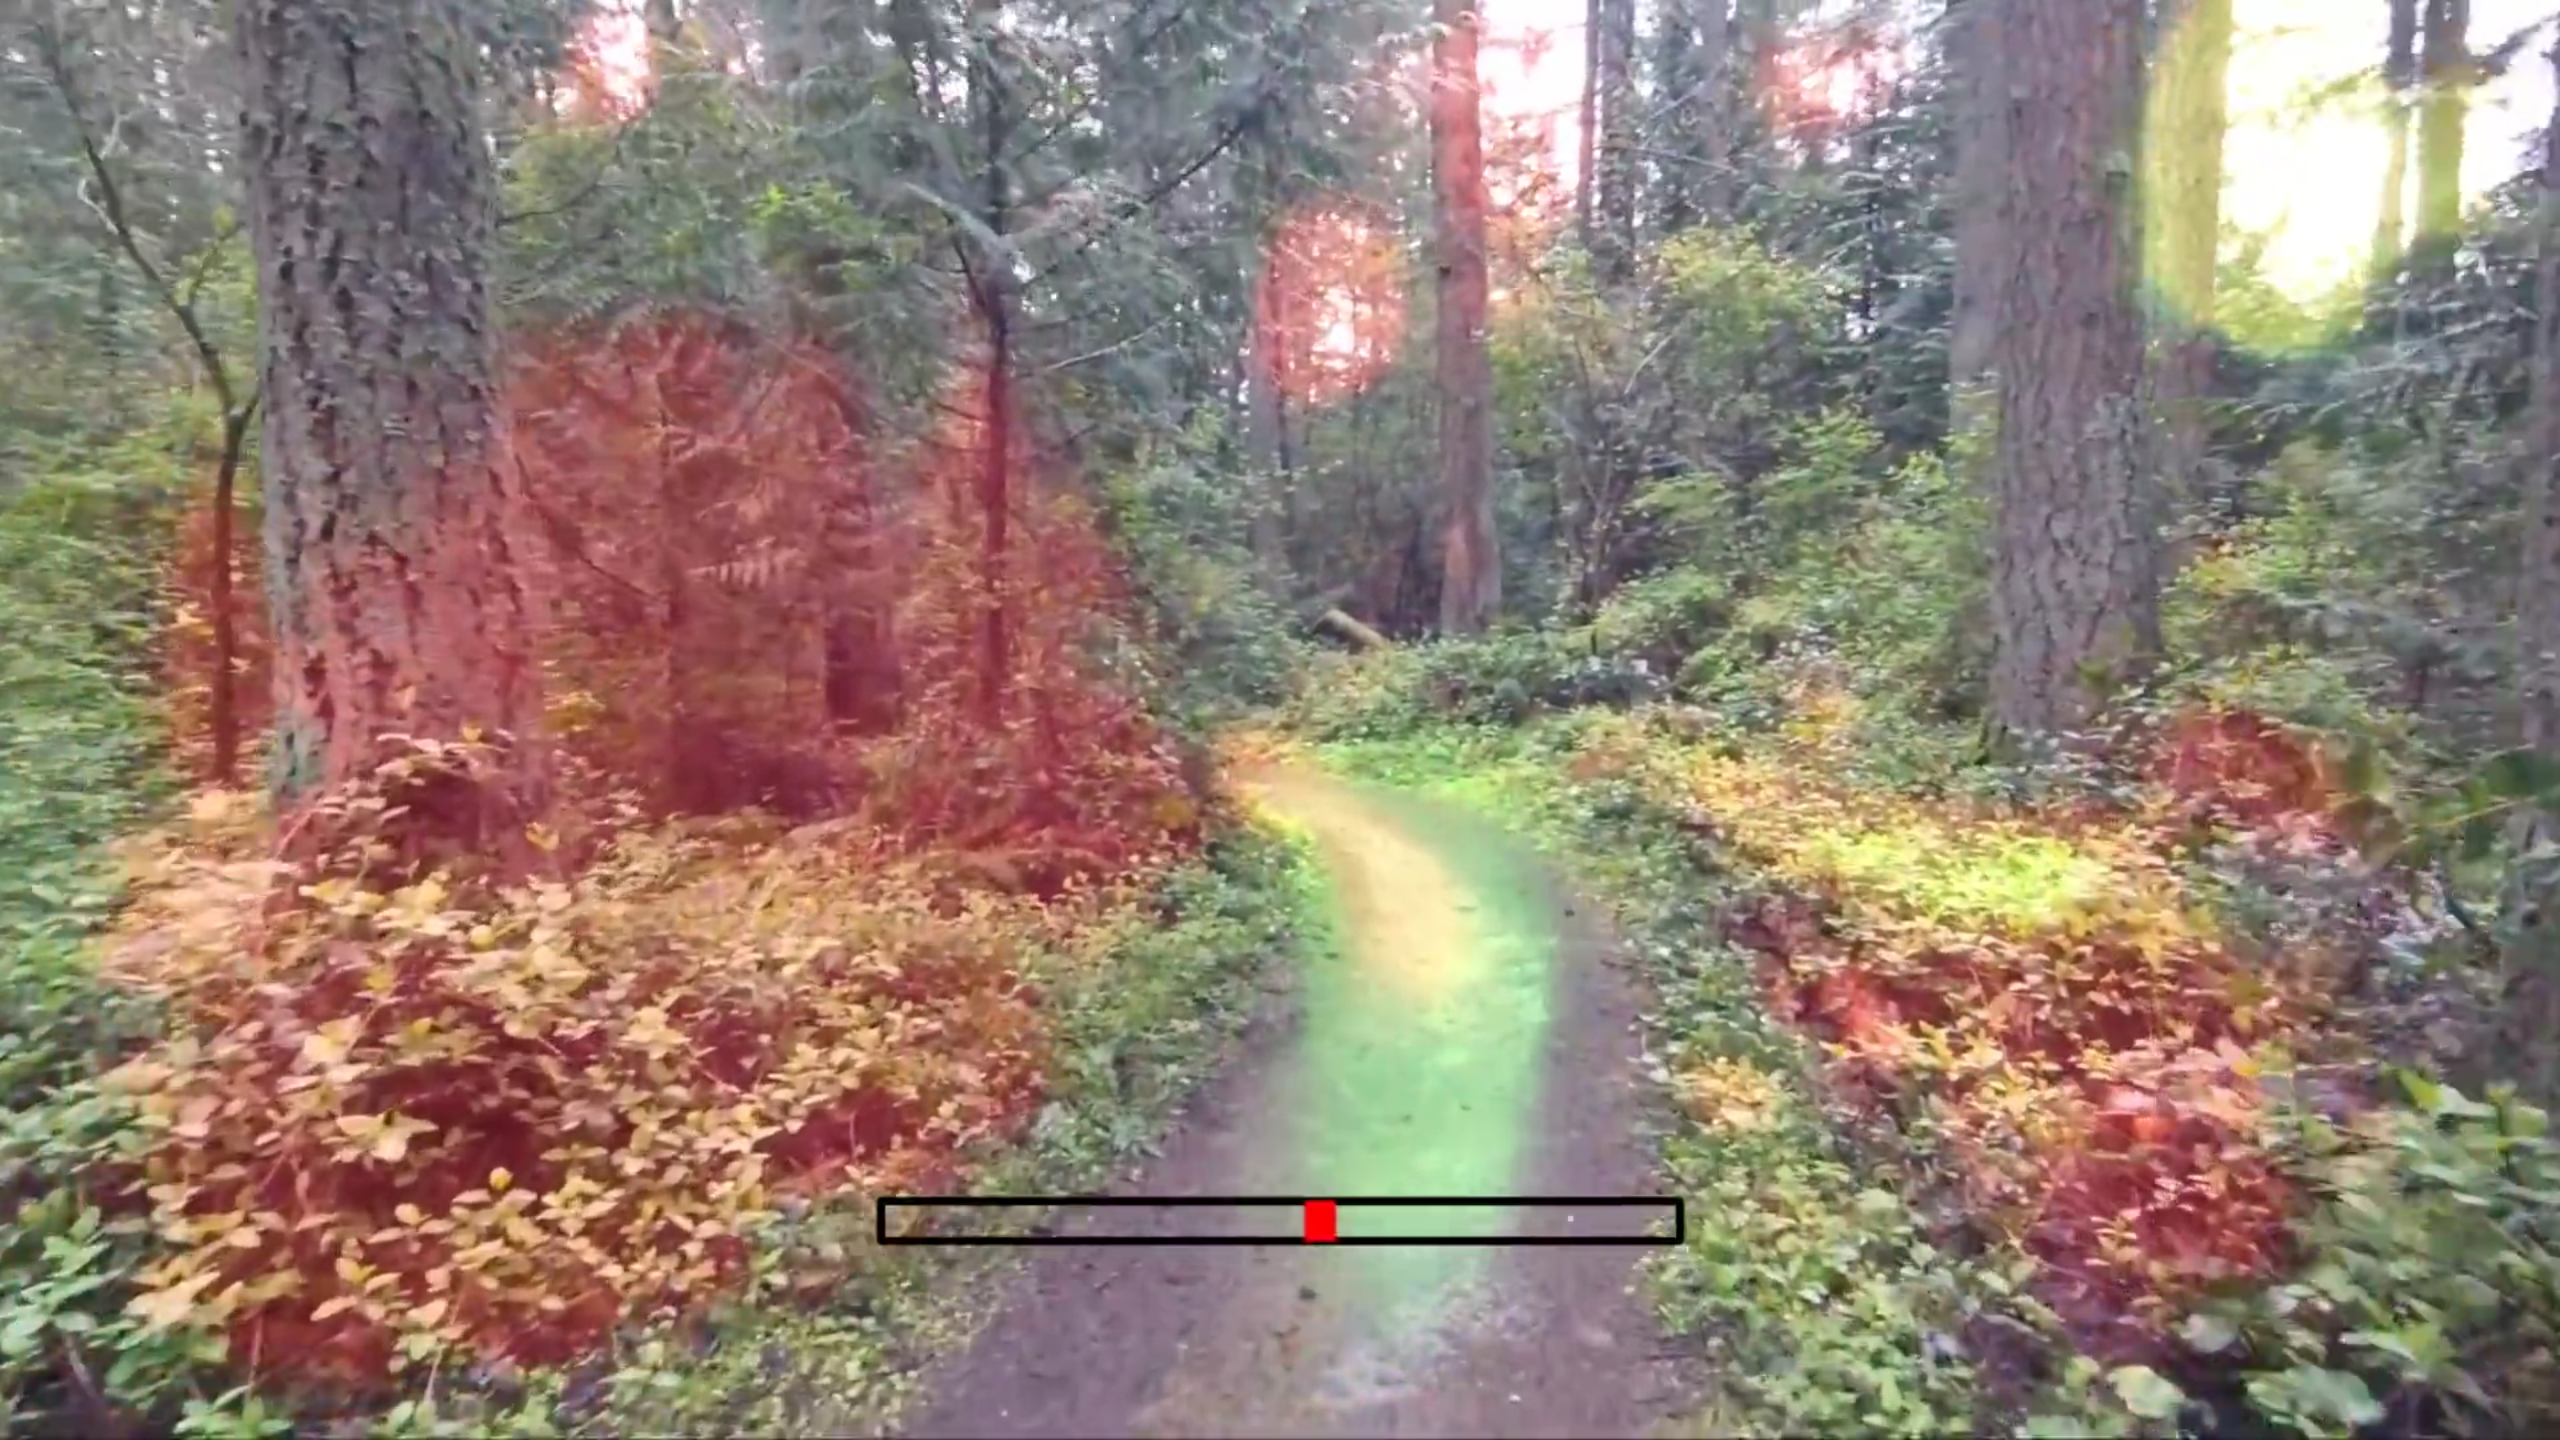
\includegraphics[width=\linewidth]{images/AutoDroneNvidia.png}}
\end{frame}

\begin{frame}{NVIDIA - Autonomous Drone video (3:10)}
	\begin{itemize}
		\item NVIDIA Jetson TX1 onboard processing, trained on videos of eight miles of trails
		%\item Sensors: PX4FLOW  optical  flow  sensor  with  sonar,and Lidar Lite V3.		
		\item Resnet-18 architecture computes view orientation and lateral offset output
		\item YOLO DNN for object detection, Visual odometry
		%\item Controller runs at 20Hz
		%\item Training data: videos shot along eight miles of trails in the Pacific Northwest, different lighting conditions with three wide-angle GoPro cameras mounted on the left, center and right of a metal bar on a mini Segway
	\end{itemize}
	\centering
	\includegraphics[width=.4\textwidth]{images/nvidia_controller.png}
	
	\tiny{\color{gray}{https://arxiv.org/pdf/1705.02550.pdf}}
	
\end{frame}

\begin{frame}{NASA JPL autonomous drone race}
        	\centering
            \href{run:./videos/NasaAutoDrone.mp4?autostart}
            {\includegraphics[width=\linewidth]{images/nasa.png}}
\end{frame}

\begin{frame}{NASA JPL autonomous drone race}
	\begin{quote}
		[...] processing is all done onboard. The team holds the drone and “walks” it through the course slowly ahead of the race to “teach” it the layout.[...] \hfill (Andrew Good, JPL, 06.12.17)
	\end{quote}

	\begin{columns}
	\begin{column}{.3\textwidth}
		\centering
		\includegraphics[width=\textwidth]{images/jpl_drone.jpeg}	
	\end{column}
	
	\begin{column}{.7\textwidth}
	\begin{itemize}
		\item Localize by comparing current sensor-input to pre-built map
		\item Google Tango technology for VR - 3D mapping
		\item Qualcomm Snapdragon Flight board is used for real-time flight control
		\item 2 wide-field-of-view-cameras: forward + downward
		\item Depth-map from motion stereo
	\end{itemize}
	\end{column}
	\end{columns}
	
	\vspace{5mm}
	\color{gray}{https://www.nasa.gov/feature/jpl/drone-race-human-versus-artificial-intelligence}
\end{frame}


\begin{frame}{Intel drone swarm}
        	\centering
            \href{run:./videos/Intel.mp4?autostart}
            {\includegraphics[width=\linewidth]{images/intel.png}}
\end{frame}


\section{Live-demo}
\begin{frame}{Livedemo}
\end{frame}

\section{Assessment}
\begin{frame}{Assessment}
\end{frame}

\end{document}
